\documentclass[journal]{IEEEtran}

\usepackage[utf8]{inputenc}
\usepackage[T1]{fontenc}
\usepackage{silence}\WarningsOff[latexfont]

\usepackage{amsmath}

\RequirePackage{tikz}[2010/10/13]
\usetikzlibrary{arrows,automata,calc,intersections,patterns,decorations.pathmorphing,decorations.pathreplacing}

\usepackage{graphicx}
\usepackage{cite}
\usepackage{url}
\usepackage[caption=false,font=footnotesize]{subfig}
\usepackage[binary-units,per-mode=symbol]{siunitx}
\sisetup{list-final-separator = {, and }}
\usepackage{booktabs}
\usepackage{pifont}
\usepackage{microtype}
\usepackage{textcomp}
\usepackage[american]{babel}
\usepackage[noabbrev,capitalise]{cleveref}
\usepackage{xspace}
\usepackage{hyphenat}
\usepackage[draft,inline,nomargin,index]{fixme}
\fxsetup{theme=color}
\usepackage{grffile}
\usepackage{xfrac}
\usepackage{multirow}
\RequirePackage{xstring}
\RequirePackage{xparse}
\RequirePackage[index=true]{acro}
\NewDocumentCommand\acrodef{mO{#1}mG{}}{\DeclareAcronym{#1}{short={#2}, long={#3}, #4}}
\NewDocumentCommand\acused{m}{\acuse{#1}}
\usepackage{upquote}
\usepackage{systeme}
\usepackage{dblfloatfix}

\graphicspath{ {./images/} }

% Keywords command
\providecommand{\keywords}[1]
{
	\small	
	\textbf{\textit{Keywords---}} #1
}


\begin{document}
\title{MQTT Bandwidth Estimation in Docker Environment}

\author{
	\IEEEauthorblockN{Simone Bernabè, Mat. number 207485\\}
	\texttt{simone.bernabe@studenti.unitn.it}
}

\makeatletter
\def\endthebibliography{%
	\def\@noitemerr{\@latex@warning{Empty `thebibliography' environment}}%
	\endlist
}
\makeatother

\markboth{MQTT Protocol - Project Course 2020}{}

\maketitle

\begin{abstract}
MQTT is an essential and growing protocol, engineered for IoT (Internet of Things) and designed to preserve power, to works well on unreliable networks, and to be a light but secure protocol. The following document is an extensive benchmark and test on MQTT bandwidth usage over some typical usage and different configurations. The objective is estimating the protocol minimum bandwidth request between sensors(\textbf{publishers}) and broker, and between broker and applications (\textbf{subscribers}). The test was led using modern technology, creating a virtual network with the usage of Docker's container, simulating the behavior of sensors, and broker, with Eclipse moquitto implementation of MQTT protocol. All the results have been resumed with plots and raw data.
\end{abstract}
\hspace{10pt}

%TC:ignore
\keywords{mqtt, bandwidth, docker}

\acresetall

\section{Introduction}
\label{sec:introduction}
MQTT is a lightweight protocol that transports messages between devices and is today widely used in the field of "Internet of Things (IoT) \cite{mqtt}." 
It's clear how this protocol represents right now state of the art for that type of connection. Still, there are no much documentation and tests on how much scalable the protocol is with different types of implementation and which is the minimum bandwidth request with a high number of elements. This work aims to characterize the traffic generated by this protocol in different configurations, both between sensors and broker, that between broker and applications. The protocol has therefore been tested with different numbers of sensors and sinks which placed before sensors, allow to convoy and parse the traffic more efficiently. Besides, the sensors have been tested using multiple messages sending patterns. 

A peculiarity of this test is the environment in which has been tested. In fact, all the test has been conducted in a virtual network created using Docker container and virtual machine based on a minimum footprint Linux image. The generated message was finally captured and analyzed using the Wireshark application. 

The document also gives a detailed insight on MQTT protocol, in all the mechanics of functioning and all the possible optimization that can be enforced to enhance the bandwidth consumption. 

In the following chapters, there are an introduction to the MQTT protocol structure as well as the functioning, 
The rest of the paper is organized as follows: Section 2 introduces the MQTT protocol, 
describing the structure and functioning,
Section 3 describes the process of preparations of the bench, which has then
been used in Section 4. Section 5 draws the Conclusions.

\section{MQTT Protocol}
MQ Telemetry Transport (MQTT) is a lightweight broker-based publish/subscribe messaging protocol designed to be open, lightweight, and easy to implement. It was designed as an extremely lightweight protocol to allow the application in remote locations with a limited internet connection and small low power devices. These principles also turn out to make the protocol ideal of the emerging “machine-to-machine” (M2M) or “Internet of Things” world of connected devices, and for mobile applications. 

The protocol was first invented by IBM in 1999 and has now become an OASIS/ISO standard with the latest release version \cite{mqtt_spec}.

The protocol runs over TCP/IP and typically on port 1883, which is assigned by the Internet
Assigned Numbers Authority (IANA). For using MQTT over SSL, port 8883 is used. 

In image \ref{fig:flow} there is a communication example, with a sensor publishing a temperature and a subscriber receiving it. 
A Packet consists of up to three parts, always in the following order, as shown below in figure \ref{fig:packet}.

\begin{figure}[h]
	\centering
	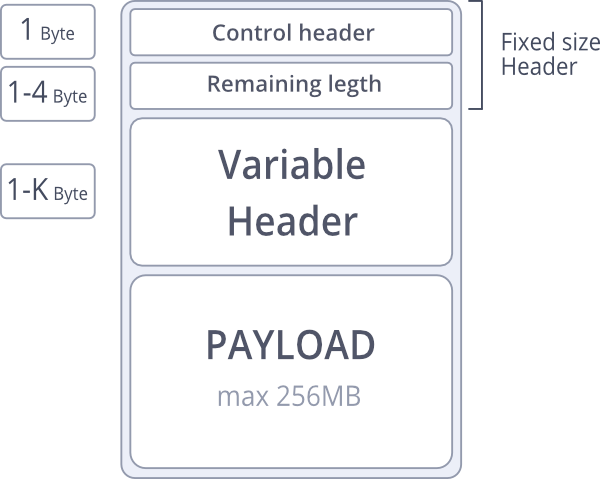
\includegraphics[width=0.38\textwidth]{mqtt_2}	
	\caption{MQTT packet format, with fixed header, variable header and payload}
	\label{fig:packet}
\end{figure}

\subsection{Fixed header}
This header is present and mandatory in all the packet types. 
Byte 1 goes to the Control field that, divided into two 4 bit fields, contains all of the protocol commands and responses. 
The first 4 most significant bits are the command or message type field, and the other 4 bits are used as control flags \cite{steven}.
Control flags include the necessary QoS (Quality of Service) selection. 

The second part (starting from Byte 2) is instead the Remaining Length, a Variable Byte Integer that represents the number of bytes remaining within the current Control Packet, including data in the Variable Header and the Payload.
\subsection{Variable header}
Some types of MQTT Control Packets contain a Variable Header component. It resides between the Fixed Header and the Payload. 
The content of the Variable Header varies depending on the packet type. The Packet Identifier field of Variable Header is common in several packet types. Other variables are set based on the type of message sent. 
For example, the publish message includes a \textbf{topic} field, which refers to the argument or directory in which the client publishes its messages. This filed has a maximum size of 65536 Byte. 

\subsection{Payload}
The last part is nothing less than the message the client wants to send. The maximum size of 256MB is limited by the 4 Byte of the Remaining length field I mentioned before. 

\begin{figure}[h]
	\centering
	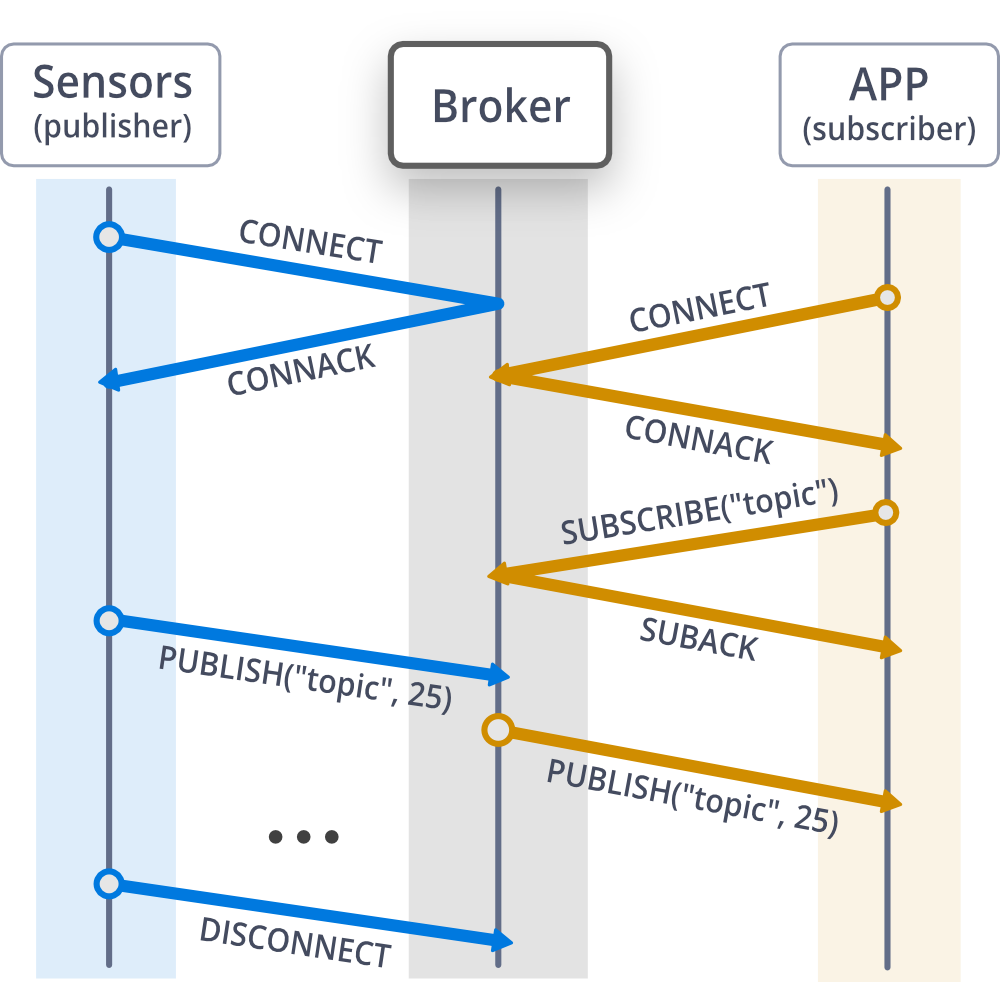
\includegraphics[width=0.4\textwidth]{mqtt}
	\caption{MQTT communication: A sensors connect to the broker and \text{publish} to a topic some value. Meanwhile, an app has connected to the broker and \textbf{subscribe} to the same topic. So, the broker forwards the message published by the sensor to the app.}
	\label{fig:flow}
\end{figure}

\section{Preparations}
To complete the bandwidth tests i tried multiple configuration and with it, i found multiple issue and tricky situation that i'll explain later on. 
The final architecture that is shown in figure \ref{fig:strut}, has $N$ sensors based on docker container and a MQTT broker on a virtual machine. The application side (subscribers) has been simulated using MQTT.x, a simple client that allow to visualize and subscribe to a broker directly. 

\begin{figure}[h]
	\centering
	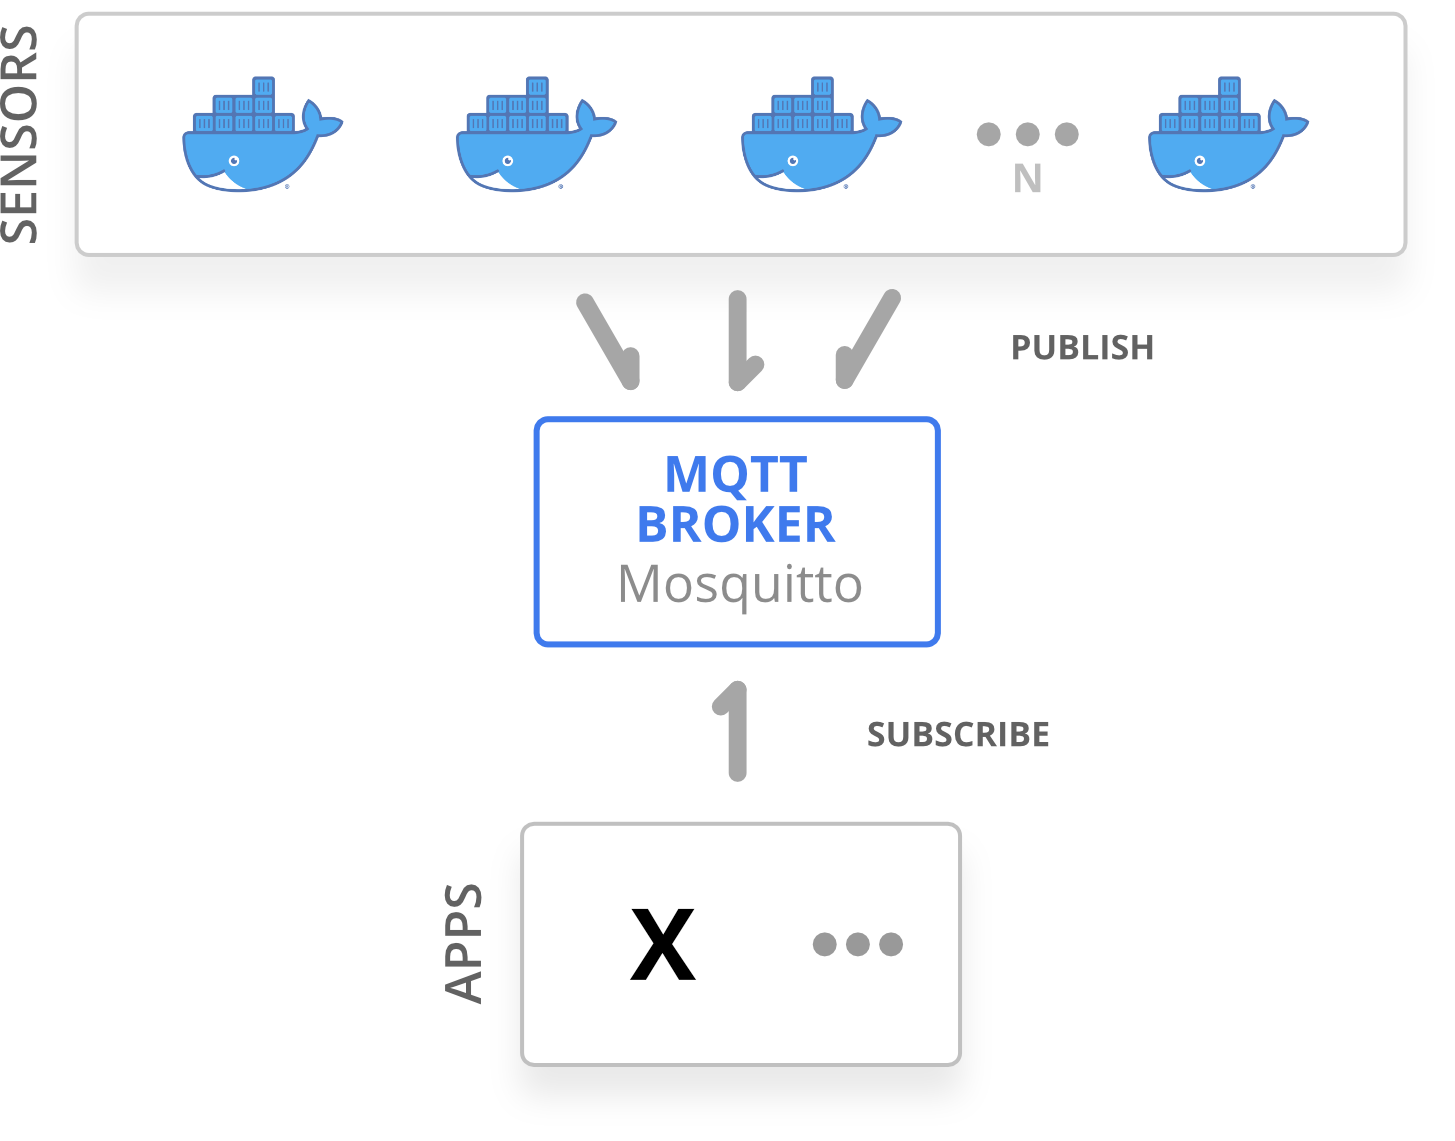
\includegraphics[width=0.4\textwidth]{struttura}
	\label{fig:strut}
	\caption{Testing architecture}
\end{figure}

\paragraph{Docker Sensors}
To simulate the sensor (publisher) I choose a minimal docker container based on Alpine linux distribution. 
An initial try was to use a simple bash script to publish on broker using the Mosquitto client commands. Unfortunetly, that command did not use session and each publish rappresent a new sending sessions. This means that every communication include a connect and a disconnect, creating an overhead due to an unnecessary message.

A library and a programming language is needed to completely take advantagess of mqtt protocol and consequentely to optimize the communication. 
Said this, I tried different language to create the sensor program. 

\begin{itemize}
	\item Python: Installing python on a container require too many disk space resources and is slower
	\item Java: This implementation is the simplest one, but since Java is running on a virtual machine, every container become too heavy on the RAM (20MB circa).
	\item C: C implementation is a little more tricky, but it does not need any installation on container and the RAM occupation once running has setted to an incredible 0.9MB. This means that simulating 100 sensors only take 90MB RAM occupation, and so gives me more flexibility on testing. 
\end{itemize}

The program consist in two modalities: 

\begin{itemize}
	\item {n}s delay: Sensors send a publish message on a given topic every {n} seconds. This make all the sensors to have the same beahviour and to have an heavy load on the bandwidth. 
	\item Realistic: This instead randomize the sending behaviour, offsetting all the sensor and creating a more realistic behaviour, close to an implementation where sensor respond to events. 
\end{itemize}

\paragraph{MQTT Broker}
To implement the MQTT broker, the Eclipse mosquitto release has been choose, that is currently one of the most used. 
An official docker image exist for mosquitto and worked just fine out of the box. 
But, for convenience Mosquitto has been installed on a Xubuntu virtual machine to better sniff on the network interface using Wireshark application. 

\section{Testing}
\begin{figure}[h]
	\centering
	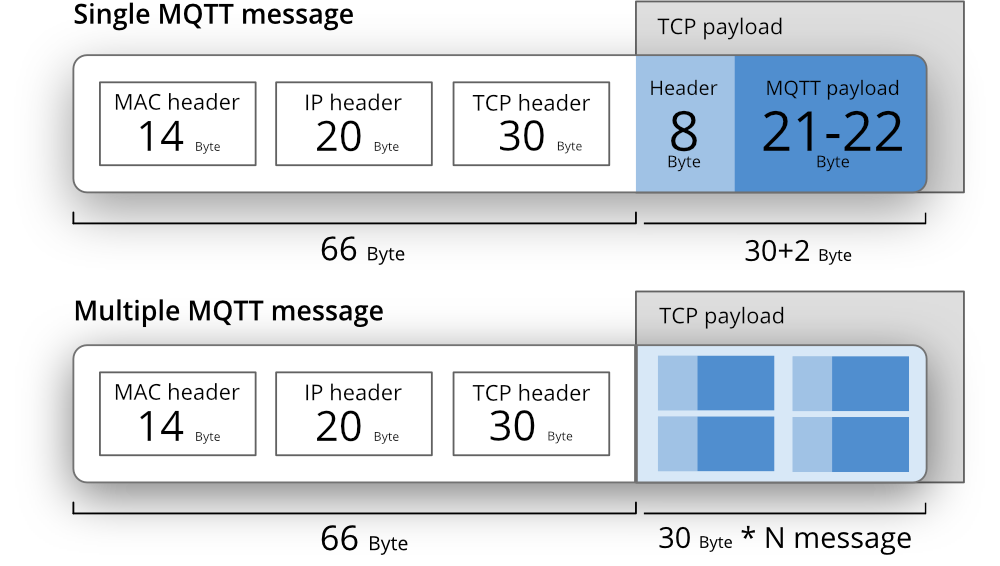
\includegraphics[width=0.4\textwidth]{mqtt_3}
	\label{fig:mqtt3}
	\caption{Overhead of the protocol aside the particular example MQTT message}
\end{figure}


\section{Conclusions}


\bibliographystyle{IEEEtran}
\bibliography{references}

\end{document}
